\documentclass[a4paper,12pt]{report}
\usepackage{adjustbox}
\usepackage[left=2.5cm,right=2.5cm,top=3cm,bottom=2.5cm]{geometry}
\usepackage{fancyhdr}
\usepackage{circuitikz} % Para dibujar circuitos
\usepackage{etoolbox}
\usepackage{multirow}
\usepackage{titlesec}
\usepackage{titling} 
\usepackage{pgfplots}

\pagestyle{fancy}
\fancyhf{} 
\fancyhead[L]{UTN-FRC}
\fancyhead[C]{Fisica Electronica: Efecto Compton}
\fancyhead[R]{2R3}
\renewcommand{\headrulewidth}{0.4pt}
\fancyfoot[C]{\vfill\thepage}
\setlength{\headwidth}{\textwidth} % Hace que el ancho del encabezado coincida con el ancho del texto
\setlength{\headheight}{15pt}  % Ajusta la altura del encabezado
\setlength{\headsep}{20pt}     % Ajusta la separación entre el encabezado y el contenido

\usepackage{titlesec}
\titleformat{\chapter}[display]
  {\normalfont\Large\bfseries}{}{0pt}{}
\titlespacing*{\chapter}{10pt}{-45pt}{10pt}

\usepackage{etoolbox} 
\makeatletter
\patchcmd{\chapter}{\thispagestyle{plain}}{\thispagestyle{fancy}}{}{} %Muestra encabezado en las páginas con \chapter
\makeatother

\titleformat{\chapter}[display]
  {\normalfont\bfseries}{}{0pt}{\huge}
\titlespacing*{\chapter}{0pt}{-30pt}{20pt}

\DeclareMathSizes{12}{13}{6}{5}

\title{%
  \fontsize{25}{0}\selectfont Universidad Tecnológica Nacional \\
  \fontsize{22}{30}\selectfont Física Electrónica \\
  \fontsize{18}{25}\selectfont TPL 4: Efecto Compton
}
\author{
Franco Palombo - 401910\\
Gaston Grasso - 401892\\
Ignacio Gil - 401891\\
Luciano Cortesini - 402719\\
}
\date{30 / 10 / 2024}

\begin{document}

\maketitle

\chapter{Introducción}
  El efecto Compton es un fenómeno que demuestra la naturaleza dual de la luz, es decir, su comportamiento tanto como
  onda como partícula.

  En esencia, el efecto Compton ocurre cuando un fotón de rayos X o gamma choca con un electrón en
  reposo y lo expulsa de su posición. Como resultado de la colisión, el fotón cede parte de su energía al electrón y
  sufre un cambio en su dirección y longitud de onda. Esta longitud de onda del fotón dispersado es mayor que la
  original, lo que implica una pérdida de energía del fotón.

  Matemáticamente, la variación de la longitud de onda se describe por la fórmula de Compton:

  $$\Delta \lambda = \lambda' - \lambda = \frac{h}{m_e \cdot c} \cdot (1 - \cos \theta)$$

  Donde:
  \begin{itemize}
    \item $\lambda$ es el cambio de longitud de onda,
    \item $h$ es la constante de planck,
    \item $m_e$ es la masa del electron,
    \item $c$ es la velocidad de la luz en el vacio,
    \item $\theta$ es el angulo de dispersion del foton.
  \end{itemize}

  Como la energia el foton es $E = hf = \frac{hc}{\lambda}$, se entiende que la energia del foton luego del choque
  es menor.

\chapter{Experiencia de laboratorio}
  \section{Instrumentos utilizados}
    Para la experiencia se utilizó un contador Geiger, este dispositivo consta de un tubo relleno de un gas. Con un hilo fino metalico a lo largo de su centro,
    al que se le aplica una diferencia de potencial con respecto al tubo. Cuando una particula atravieza el tubo desprende electrones de
    de los atomos del gas, los cuales son atraidos hacia el hilo por el campo electrico generado. De esta forma, cada particula que pasa a travez del tubo produce
    un pulso electrico, permitiendo su detección. Este instrumento no proporciona información sobre el tipo de radiación o su energía, simplemente cuenta la cantidad
    de particulas que atraviezan el tubo en una determinada base de tiempo.

    \begin{figure}[h]
        \centering
        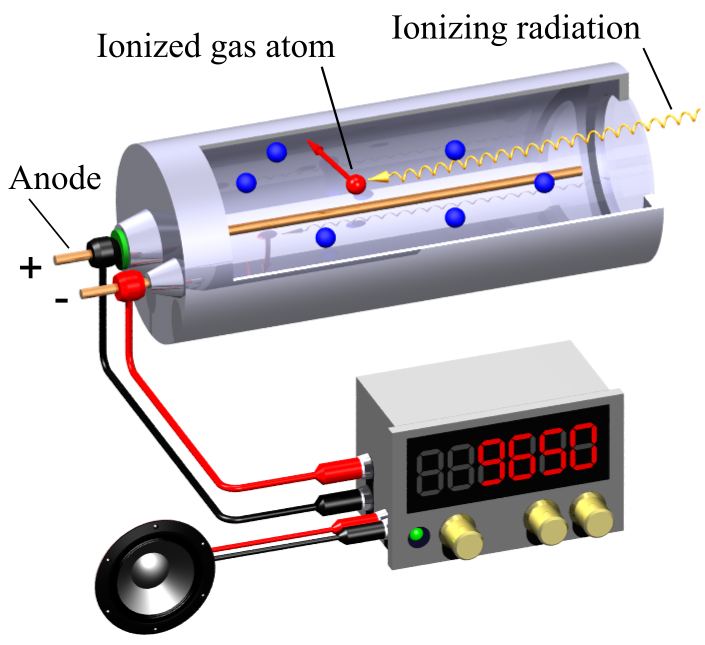
\includegraphics[width=0.5\textwidth]{images/gmCounter.png}
        \caption{Diagrama del contador Geiger Muller}
        \label{fig:etiqueta}
    \end{figure}

  \newpage
  \section{Mediciones}
    En el laboratorio se armó la siguiente disposición:
    \begin{figure}[h]
        \centering
        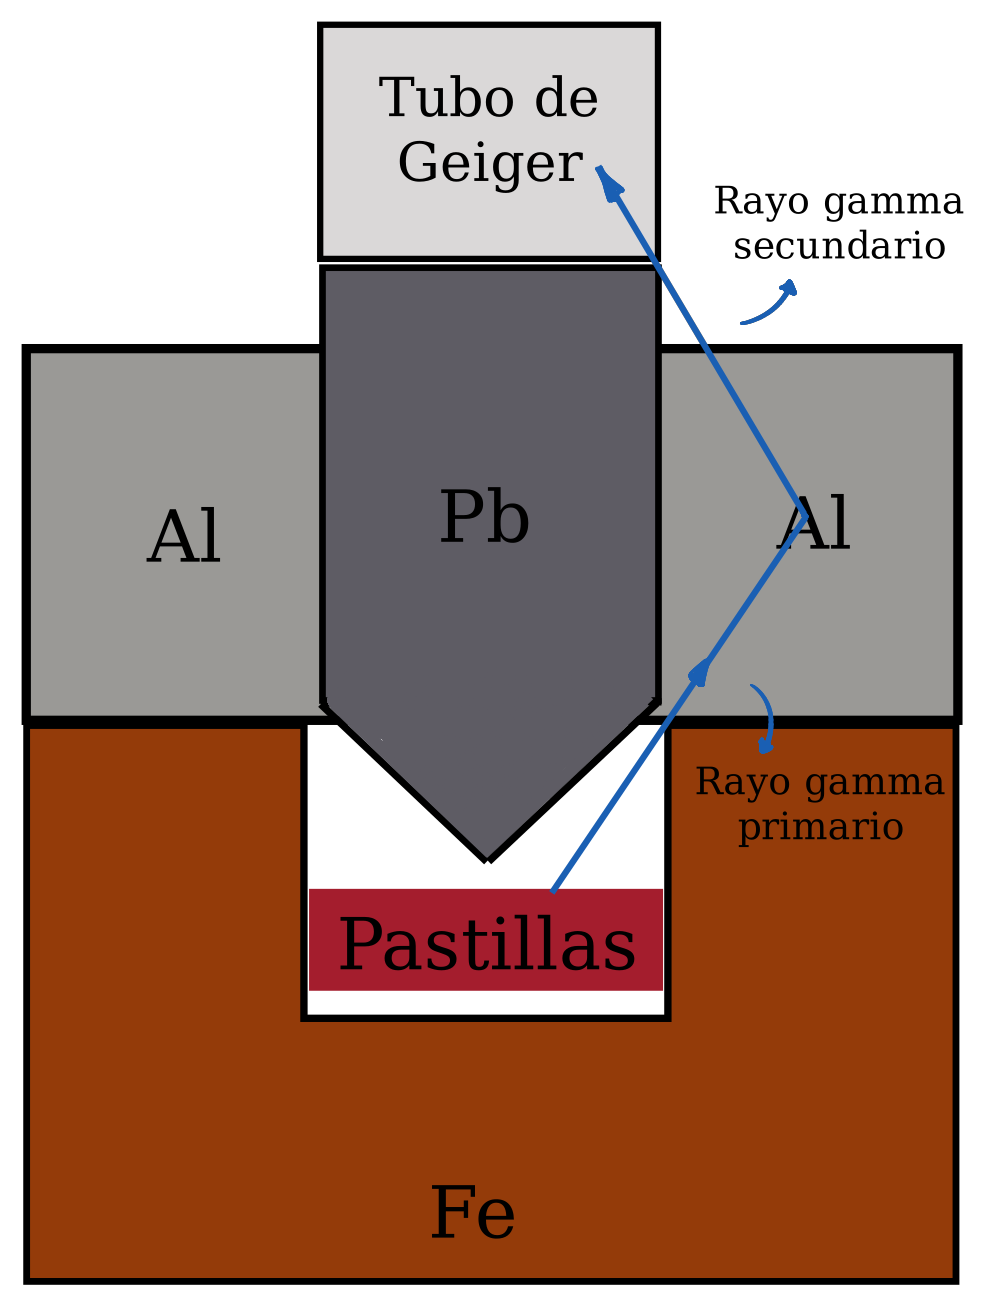
\includegraphics[width=0.5\textwidth]{images/diagrama.png}
        \caption{Diagrama del contador Geiger Muller}
        \label{fig:etiqueta}
    \end{figure}

    La finalidad es medir la radiación gamma generada por las pastillas radioactivas luego de ser dispersadas por el aluminio(dispersor de compton)
    a travez del efecto Compton. El tubo de plomo cumple la funcion de evitar que la radiación viaje directamente hacia el tubo de Geige-Muller, y
    que toda la radiación sea procedente de la sustancia difusora.
    Las pastillas radioactivas utilizadas en la expieriencia fueron:
    \begin{itemize}
        \item Bario 133
        \item Cadmio 109
        \item Cesio 137
        \item Cobalto 60
        \item Cobalto 57
        \item Magnesio 54
        \item Sodio 22
        \item Zinc 65
    \end{itemize}
    El contador de Geiger se configuró con un voltaje de 900V y una base de tiempo de 5 minutos.
    Se realizaron 4 mediciones con distintas disposiciones:
    \begin{enumerate}
        \item Con un anillo de plomo entre los cuerpos de hierro y alumnio. Lectura: 108
        \item Con un segundo anillo de aluminio sobre el anterior. Lectura: 154
        \item Con un anillo de plomo sobre el cuerpo de aluminio. Lectura: 132
        \item Con dos anillos de plomo sobre el cuerpo de aluminio. Lectura: 116
    \end{enumerate}
\chapter{Conclusión}

    Se logró observar y analizar la dispersión de los fotones
  gamma al interactuar con un material difusor, como el aluminio. A través del uso del contador Geiger-Müller, se
  registraron los niveles de radiación dispersada, demostrando cómo los fotones, al ceder parte de su energía a los
  electrones en reposo, cambiaron su dirección y energía.

  Los resultados obtenidos confirman la teoría del efecto Compton, evidenciada por el cambio en las lecturas de
  radiación en función de las distintas configuraciones experimentales. La variación en las mediciones muestra cómo la
  presencia de distintos materiales y disposiciones afecta la cantidad de fotones dispersados que llegan al detector.
  El uso de anillos de plomo, en particular, ayudó a atenuar la radiación directa, permitiendo un análisis más preciso
  de la radiación dispersada.

  Además, la diferencia en las lecturas con y sin el dispersor de aluminio evidencia la transferencia de energía de los
  fotones a los electrones, un aspecto clave del fenómeno que sustenta la naturaleza corpuscular de la luz.

\end{document}
